

\documentclass[DIV=calc, paper=a4, fontsize=11pt]{scrartcl}
\usepackage{makeidx}
\usepackage{graphicx}
\usepackage{flushend}
\usepackage{amssymb}


\usepackage{lmodern}
\usepackage[left=1.5cm,right=1.5cm,top=2.5cm,bottom=2cm]{geometry}
\usepackage{float}		
\bibliographystyle{plain} 
\pagestyle{plain} 
\pagenumbering{arabic}
\usepackage{fancyhdr} 	
\usepackage[T1]{fontenc}
\usepackage[utf8]{inputenc}
\usepackage[spanish]{babel}
\usepackage[spanish,es-tabla]{babel}
\usepackage{hyperref}
\usepackage{graphicx}
\usepackage{siunitx}
\usepackage{lipsum}
\usepackage[protrusion=true,expansion=true]{microtype}
\usepackage{amsmath,amsfonts,amsthm}
\usepackage[svgnames]{xcolor}
\usepackage[svgnames]{xcolor}
\usepackage{booktabs}
\usepackage{fix-cm}
\usepackage{multicol}
\usepackage{url}
\usepackage{cancel}
\usepackage{subfig}
\bibliographystyle{unsrt}

\newenvironment{Figura}
  {\par\medskip\noindent\minipage{\linewidth}}
  {\endminipage\par\medskip}

\usepackage{sectsty}
\allsectionsfont{\usefont{OT1}{phv}{b}{n}}
\usepackage{fancyhdr}
\spanishdecimal{.}
\pagestyle{fancy}
\usepackage{lastpage}
\lhead{}
\chead{}
\rhead{}
\lfoot{}
\cfoot{}
\rfoot{\footnotesize Page \thepage\ of \pageref{LastPage}}
\renewcommand{\headrulewidth}{0.0pt}
\renewcommand{\footrulewidth}{0.4pt}
\usepackage{lettrine}
\newcommand{\initial}[1]{\lettrine[lines=3,lhang=0.3,nindent=0em]{
\color{DarkGoldenrod}{\textsf{#1}}}{}}
\usepackage{titling}
\newcommand{\HorRule}{\color{DarkGoldenrod} \rule{\linewidth}{1pt}}
\pretitle{\vspace{-120pt} \begin{flushleft} \HorRule \fontsize{22}{35} \usefont{OT1}{phv}{b}{n} \color{DarkRed} \selectfont}
\title{Reporte 5. \\ %Aquí va el nombre de la práctica 
Espejos} %Numero de la práctica 
\posttitle{\par
\end{flushleft}
\vskip 0.5em}
\preauthor{\begin{flushleft}\large \lineskip 0.5em \usefont{OT1}{phv}{b}{sl} \color{DarkRed}}
\author{Angel Yair García Pérez \\
Misael Iván Macías Márquez\\
Teodora Irene Ortíz Cruz\\
\small{teodora625@ciencias.unam.mx}\\}
\postauthor{\footnotesize \usefont{OT1}{phv}{m}{sl} \color{Black}
\vspace*{0.1cm} 
Facultad de Ciencias, UNAM
\par\end{flushleft}\HorRule}
\date{25 de Abril de 2022\\Semestre 2022-2}
\begin{document}
\maketitle
\definecolor{carmine}{rgb}{0.59, 0.0, 0.09}
\begin{abstract}

  \textcolor{carmine}{Resumen:} Se comprobaron las leyes de espejos planos y cóncavos propuestas en la literatura. Se midieron las distancias objeto e imagen y las alturas de cada uno. Con el espejo plano se obtuvo que $o=(50\pm0.5)\hspace{0.1cm}\text{mm}$ e $i=(49\pm1)\hspace{0.1cm}\text{mm}$. Con los datos medidos en la segunda parte se tuvo que la  posición del foco del espejo era $\mathbf{(9.901 \pm 0.098)\hspace{0.1cm} \text{cm}}$ con discrepancia de $\mathbf{1.01 < 2}$ y un radio de $\mathbf{(19.802 \pm 0.196)\hspace{0.1cm} \text{cm}}$ con discrepancia de $\mathbf{1.01<2}$  comparados con los valores de fabrica se obtuvo una incertidumbre relativa para el foco y el radio de $0.98\%$ lo cual es un resultado satisfactorio. Por ultimo, con la medidas del esferómetro se obtuvo un radio de $\mathbf{(19.071 \pm 0.641)\hspace{0.1cm} \text{cm}}$ con error de $\mathbf{1.45<2}$ y un foco en  $\mathbf{(9.536 \pm 0.321)\hspace{0.1cm} \text{cm}}$ discrepancia de $\mathbf{1.45<2}$ e incertidumbre relativa de $3.36\%$ para ambos y también es un resultado satisfactorio.
\end{abstract}
\section*{\textcolor{carmine}{Introducción}}
 El propósito de este trabajo es caracterizar los espejos planos y cóncavos comprobando que cumplen con el modelo propuesto por la literatura\cite{Manual}. La importancia de este trabajo se centra en estudiar el comportamiento de las imágenes producidas por los distintos  espejos y verificar que el modelo teórico cumple con las observaciones experimentales. En particular para el espejo cóncavo se calculará el radio de curvatura y el foco del espejo por medio de la ecuación del espejo y un esferómetro \cite{article}. Se compararan los resultados con los datos de fabrica. Se espera que se cumpla la teoría propuesta y a partir de los datos obtener un radio de curvatura con valor cercano a $20\hspace{0.1cm}\text{cm}$ y un foco en $10\hspace{0.1cm}\text{cm}$. 
 \subsection*{\textcolor{carmine}{Espejo plano.}}
Un espejo plano es una superficie reflectora plana, si frente a el se coloca un objeto de altura $h$ a una distancia $o$ como se muestra en la Figura 1 los rayos de luz serán reflejados y se obtendrá una imagen, para un observador de frente parecerá que la imagen $P'$ es la que emite los rayos, la cual está a una distancia $i$ y altura $h'$\cite{book}. Utilizando algunas relaciones entre los triángulos se obtiene que la imagen situada frente a un espejo plano esta a la misma distancia que la del objeto frente a espejo\cite{Manual}, es decir
\begin{equation}
    o=i
\end{equation}
\begin{figure}[H]
    \centering
    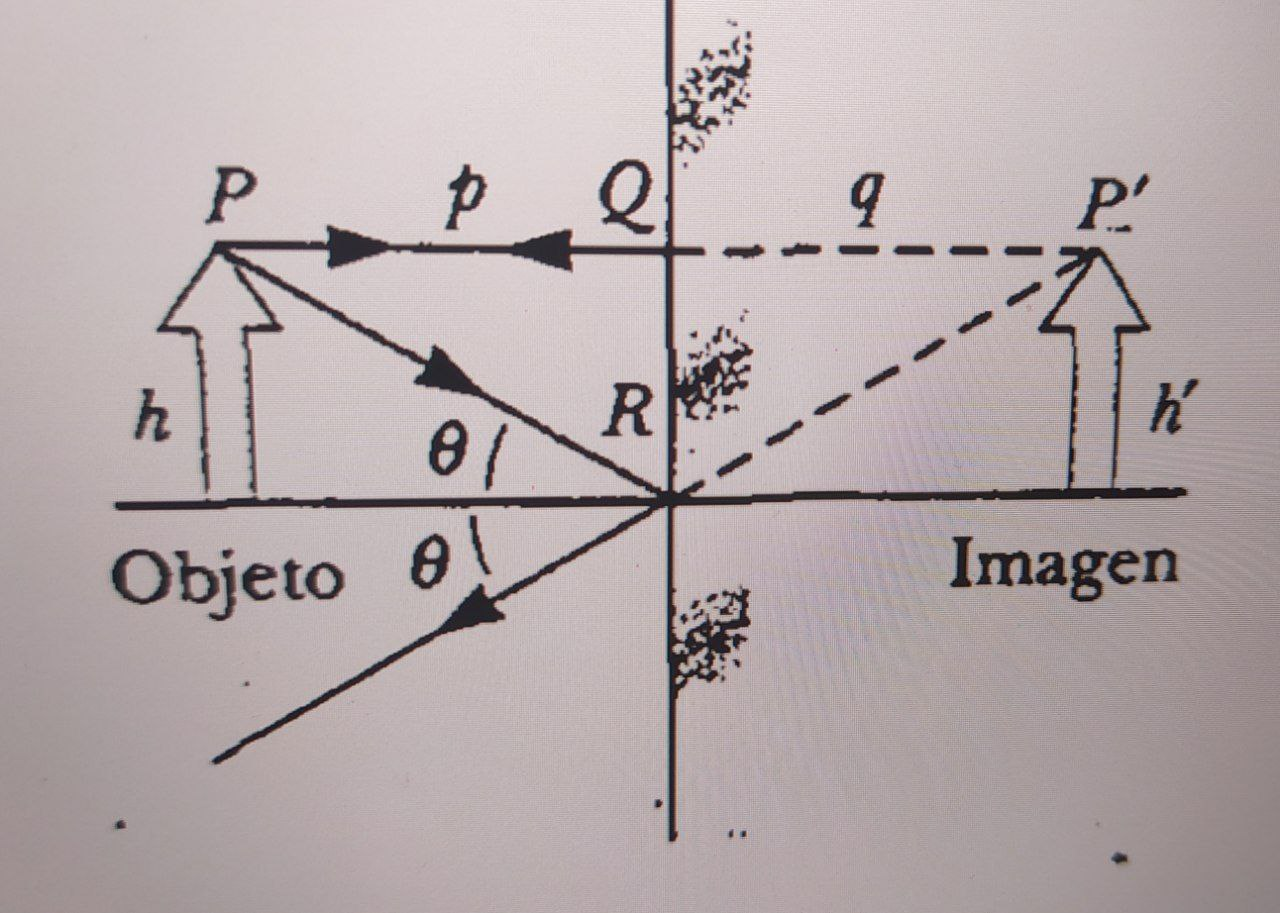
\includegraphics[width=7cm]{fotos/introducción/photo_2022-04-24 17.05.39.jpeg}
    \caption{\textbf{Diagrama de espejo plano.} La línea de en medio representa al espejo, mientras que p es la distancia objeto-espejo y q es la distancia espejo-imagen\cite{book}.}
    \label{fig:my_label}
\end{figure}
\subsection*{\textcolor{carmine}{Espejo cóncavo.}}
Un espejo esférico cuya luz se refleja en la superficie interior es llamado espejo cóncavo. Tiene un radio de curvatura $R$ y un foco $f$. Si se coloca un objeto frente al espejo como se muestra en la Figura 2 se formará una imagen frente al espejo y haciendo uso de la aproximación paraxial y las relaciones entre triángulos se obtiene que la ecuación que caracteriza a este espejo es \cite{book}
\begin{equation}
    \frac{1}{o} = -\frac{1}{i} + \frac{1}{f} = -\frac{1}{i} + \frac{2}{R}
\end{equation}
Utilizando la misma geometría del diagrama se puede llegar a que hay un factor de proporcionalidad denominado magnificación lateral que esta dada por
\begin{equation}
  M=\frac{h'}{h}=-\frac{i}{o}
\end{equation}
\begin{figure}[H]
    \centering
    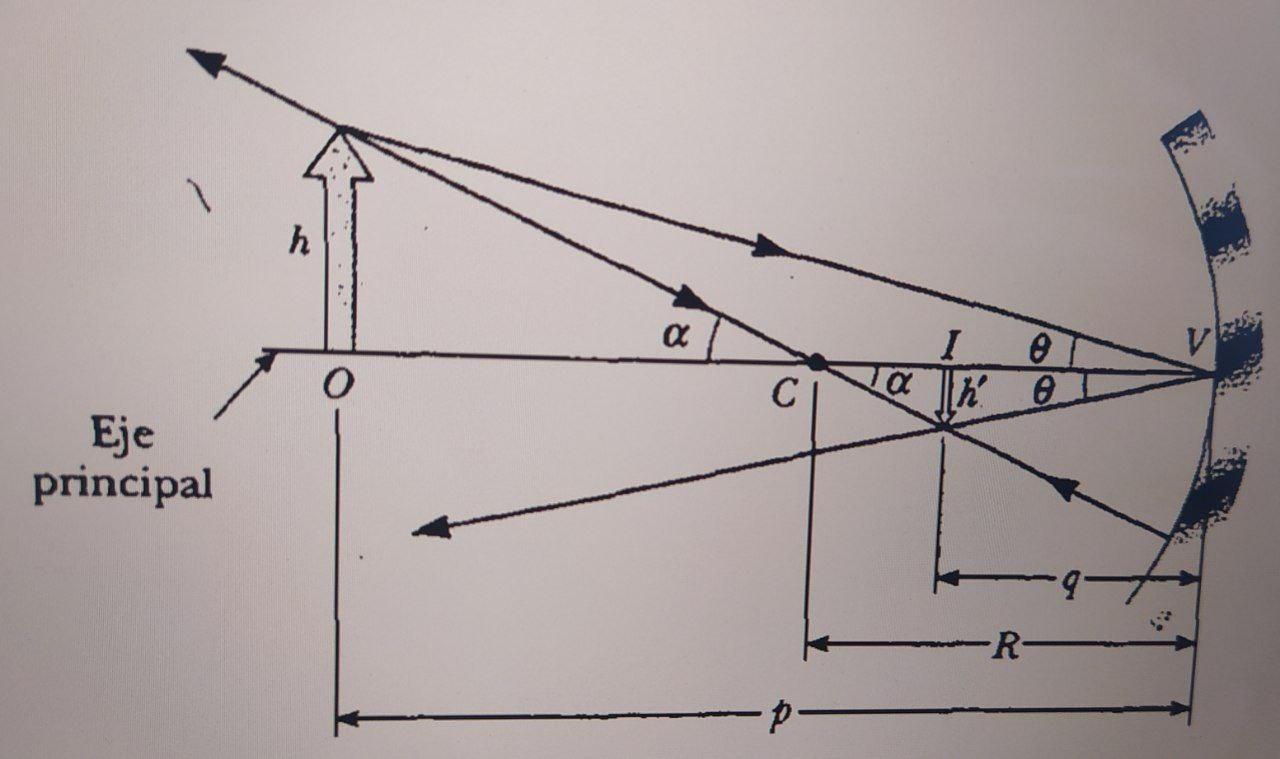
\includegraphics[width=7cm]{fotos/introducción/photo_2022-04-24 17.05.43.jpeg}
    \caption{\textbf{Diagrama de espejo cóncavo.} La $O$ representa al objeto colocado frente a espejo y la imagen es $I$. En la figura también se observa la distancia $p$ objeto-espejo y $q$ imagen-objeto\cite{book}.}
    \label{fig:my_label}
\end{figure}
\subsection*{\textcolor{carmine}{Esferómetro.}}
Es un instrumento de laboratorio que sirve para medir el radio de curvatura, consiste en un tornillo insertado en un pequeño trípode equilátero o anular que cuenta con una escala graduada vertical. Para obtener su modelo matemático consideremos la Figura 3 y aplicando teorema de pitágoras se puede obtener que la ecuación para obtener el radio de curvatura es \cite{article}
\begin{equation}
    R= \frac{a^2}{2h}+\frac{h}{2}
\end{equation}
\begin{figure}[H]
    \centering
    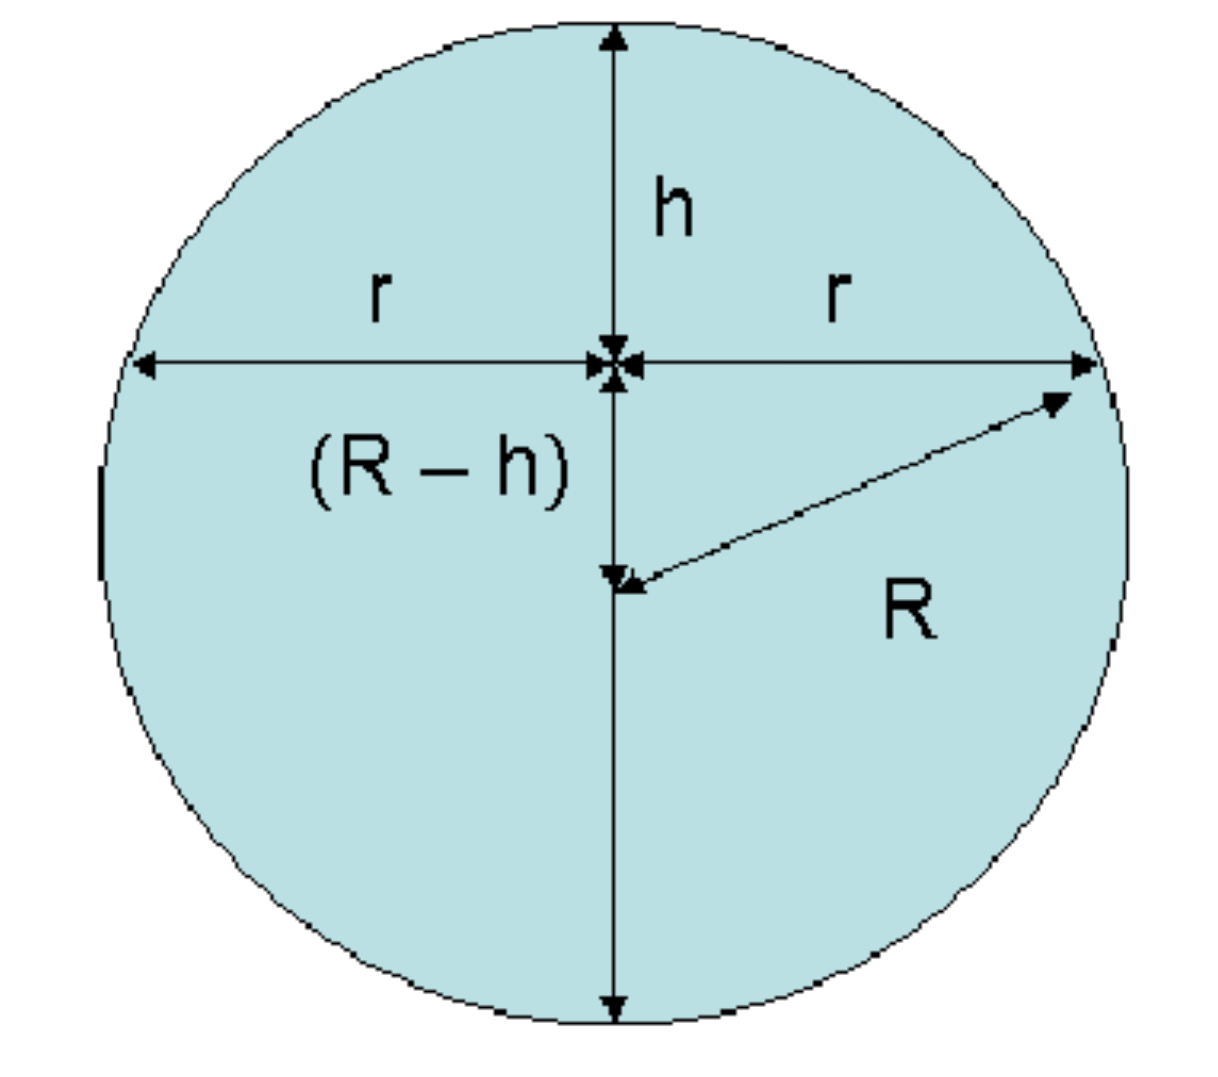
\includegraphics[width=7cm]{fotos/introducción/915DB293-CFE6-4BEF-882D-1ECBF124F44F.jpeg}
    \caption{\textbf{Diagrama del esferómetro.} En este diagrama se observa la geometría implicada en las ecuaciones del esferómetro para obtener la ecuación (4) \cite{article}}
    \label{fig:my_label}
\end{figure}
\section*{\textcolor{carmine}{Desarrollo Experimental.}}
\subsection*{\textcolor{carmine}{Parte I}}
 Sobre la mesa de trabajo se acomodó una hoja de papel milimétrico, un tornillo pequeño, un espejo plano y una regla/mira. Se trazó una línea en la mitad de la hoja y sobre ella se colocó el espejo plano, luego se buscó un punto donde el reflejo del objeto se apreciará bien desde varias posiciones, el punto fue marcado como se muestra en la Figura 4.  Se ubicaron tres puntos distintos de observación y en cada uno se colocó la mirilla con la que se trazaron las líneas correspondientes, el punto de cruce de las líneas es aproximadamente la posición de la imagen del objeto generada por el espejo. Se detectó que la hoja milimétrica tenía una incertidumbre dada por $\sigma_{a}=0.05\hspace{0.1cm}\text{mm}$ la cual sería la incertidumbre de la distancia objeto.
\begin{figure}[H]
    \centering
    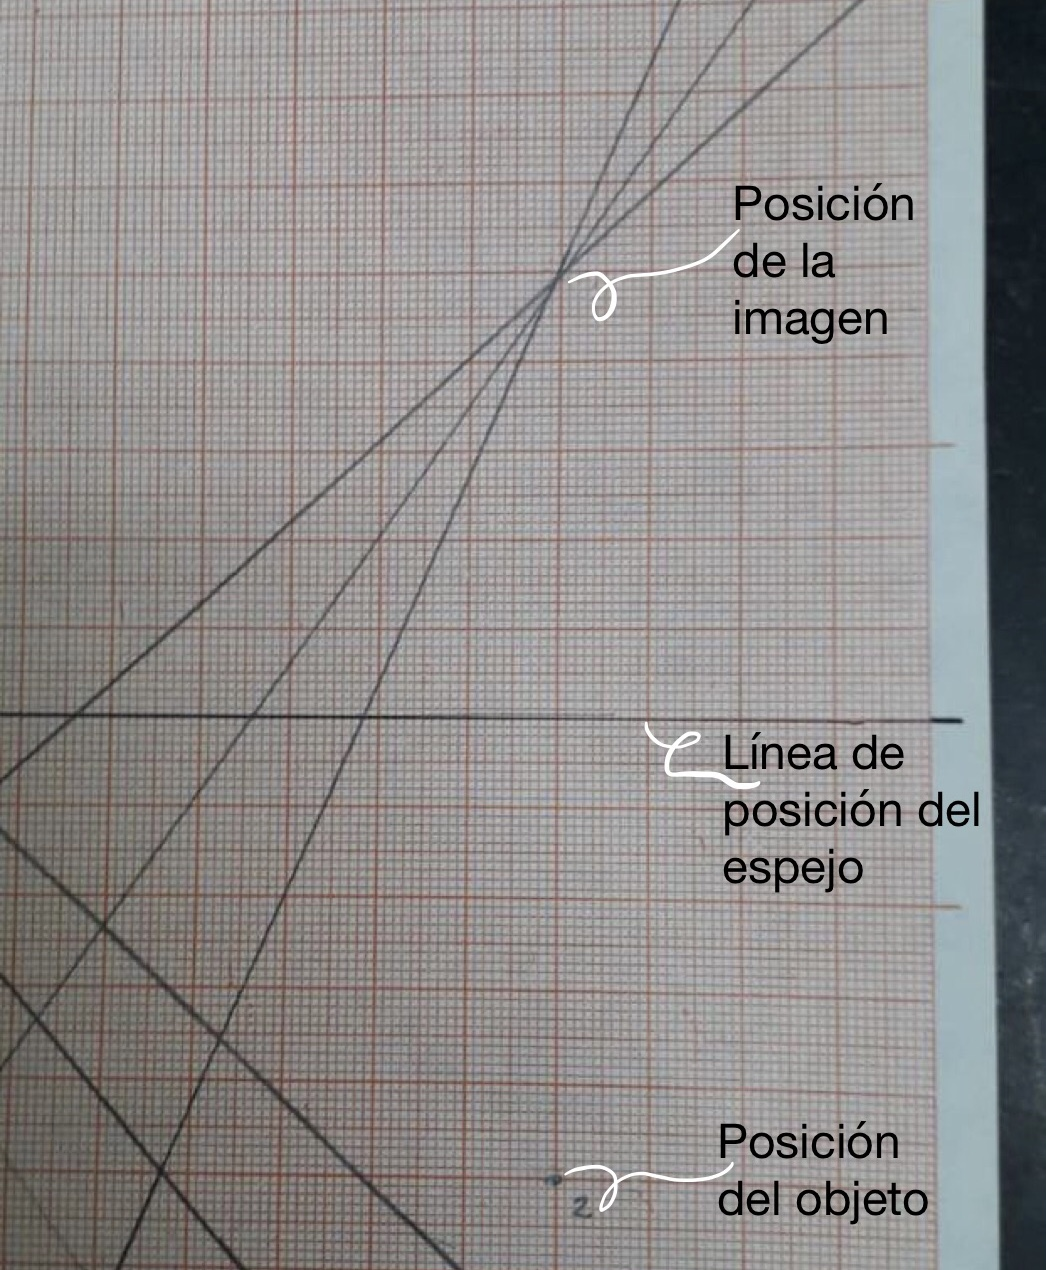
\includegraphics[width=7cm]{fotos/introducción/885C2AA8-BBFB-4541-94BC-36BB5FACD629.jpeg}
    \caption{\textbf{Diagrama del primer experimento.} La línea de posición del espejo es la línea sobre la que se colocó el espejo, el objeto fue colocado en el punto denominado posición de objeto y la distancia imagen espejo esta dada por la distancia entre la linea de posición del espejo y el punto de cruce de las tres líneas.}
    \label{fig:my_label}
\end{figure}
\subsection*{\textcolor{carmine}{Parte II}}
%Se utilizó el riel óptico con escala en el se colocó un espejo cóncavo, una pantalla y una fuente de luz led plana como se muestra en la Figura 5. Se colocó la pantalla cerca del espejo para evitar las aberraciones en las primeras medidas y se movió la luz led a 4 posiciones distintas. Se registraron los datos de la altura proyectada en la pantalla, la altura original y las distancias a las que se encontraba el  objeto y la imagen. En esta parte la incertidumbre de las alturas del objeto estuvieron dadas por $\sigma_{a}=\pm0.01\hspace{0.1cm}\text{mm}$, la incertidumbre para las alturas del la imagen fue dada por $\sigma_{a}=\pm0.02\hspace{0.1cm}\text{mm}$, la distancia objeto tuvo la incertidumbre de la mínima escala entre dos del riel óptico siendo de $\pm0.05\hspace{0.1cm}\text{cm}$ para la distancia imagen cambió debido a que en algunos casos se tuvo un intervalo de medidas a estos se les asignó como incertidumbre la diferencia de los valores medidos como se muestra en el cuadro 2 (ver apéndice).
Se utilizó el riel óptico con escala sobre el que se colocó un espejo cóncavo, una pantalla y una fuente de luz led plana como se muestra en la Figura 5. Se movió la luz led a diferentes posiciones, después se movió la pantalla hasta que la imagen formada fuera clara. En algunas posiciones de la fuente de luz se tuvo una incertidumbre de definición $\sigma_{def}$. Para 4 posiciones distintas del led se registró la altura de la imagen proyectada en la pantalla y la altura del objeto original. La incertidumbre de las alturas del objeto estuvo dada por $\sigma_{a}=\pm0.01\hspace{0.1cm}\text{mm}$, asociada a la incertidumbre de la escala integrada en el led, la incertidumbre para las alturas del la imagen fue dada por $\sigma_{a}=\pm0.02\hspace{0.1cm}\text{mm}$, corresponde a la incertidumbre del vernier, la distancia objeto tuvo la incertidumbre de la mínima escala del riel óptico entre dos siendo de $\sigma_{ap}=\pm0.05\hspace{0.1cm}\text{cm}$, para la distancia imagen la incertidumbre cambió debido a que $\sigma_{def}$ dependía de la posición del led.




\begin{figure}[H]
    \centering
    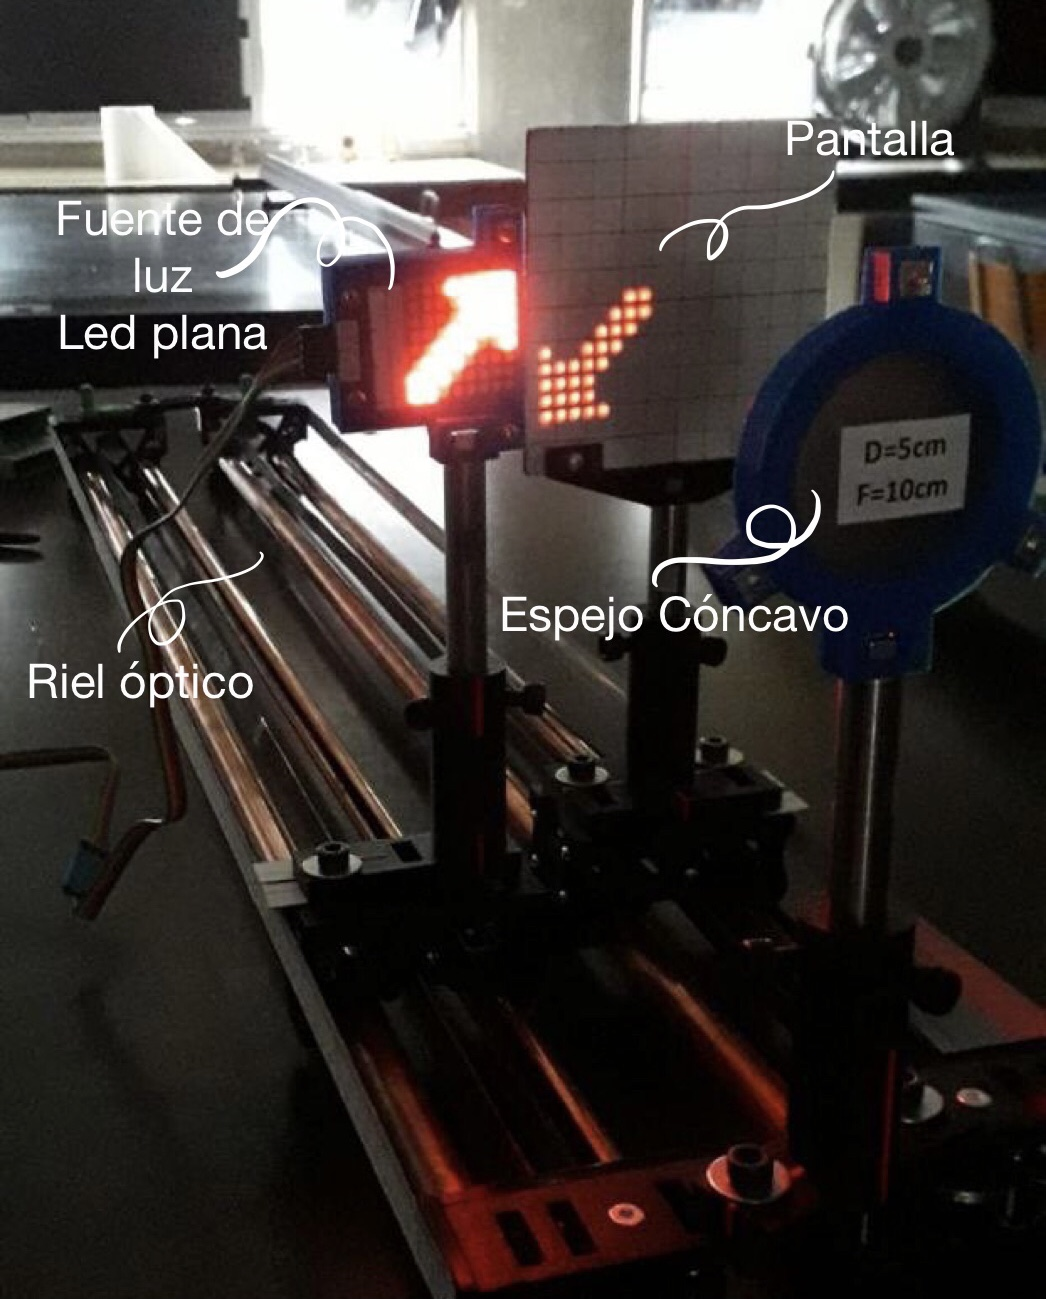
\includegraphics[width=8cm]{fotos/D2FD62FA-C29E-4E97-AB6B-5FD1C6AE4100.jpeg}
    \caption{\textbf{Arreglo experimental.}}
    \label{fig:my_label}
\end{figure}
\subsection*{\textcolor{carmine}{Parte III}}
Se colocó sobre la mesa óptica del laboratorio un esferómetro  se giró hasta que el tornillo tocara con la superficie de la mesa y se estableció que el cero se encontraba en $0.003\hspace{0.1cm}\text{cm}\pm0.001\hspace{0.1cm}\text{cm}$, se identificó que el esferómetro tenía una incertidumbre de $\sigma_{a}=0.001\hspace{0.1cm}\text{cm}$. Luego se colocó sobre el espejo y se giró hasta tocar con la superficie del espejo, se contaron el número de vueltas. Con un vernier se midió la altura y se determinó que la incertidumbre estaba dada por $\sigma_{a}=0.005\hspace{0.1cm}\text{cm}$, el procedimiento se repitió 3 veces con los mismos instrumentos. 
\newpage
\section*{\textcolor{carmine}{Resultados y Discusión.}}

\subsection*{\textcolor{carmine}{Espejo plano.}}

La distancia objeto medida con su incertidumbre de apreciación es:

\begin{equation*}
    o= (50 \pm 0.5) \hspace{0.1cm} \text{mm}
\end{equation*}

%La distancia imagen medida con su incertidumbre como el radio de la bola generada por las 3 mediciones hechas es:
La distancia imagen medida con su incertidumbre como la distancia entre las $2$ mediciones mas lejanas entre $2$ es:
\begin{equation*}
    i= (49 \pm 1) \hspace{0.1cm} \text{mm} 
\end{equation*}
Con base a lo anterior se puede decir que se cumple el modelo que caracteriza a un espejo plano (1). 

\subsection*{\textcolor{carmine}{Espejo cóncavo.}}

\begin{figure}[H]
    \centering
    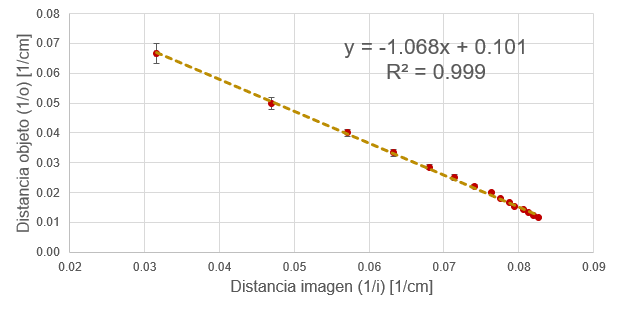
\includegraphics[scale=0.8]{graficas/grafica espejo concavo.PNG}
    \caption{\textbf{Gráfica de distancia imagen vs distancia objeto.} Gráfica de $\frac{1}{o}$ vs $\frac{1}{i}$, el ajuste se hizo con los datos del cuadro 2 }
    \label{fig:my_label}
\end{figure}

Con el ajuste se obtuvo que la ordenada al origen con su incertidumbre estadística es:

\begin{equation*}
    b=(0.101 \pm 0.001) \frac{1}{\text{cm}}
\end{equation*}

que por la ecuación 2, el foco y el radio de curvatura del espejo son:

\begin{equation*}
    f=\frac{1}{b}   \hspace{3cm} R = \frac{2}{b} \hspace{0.1cm}
\end{equation*}
\begin{equation*}
    \hspace{1.7cm}= 9.901 \hspace{0.1cm} \text{cm}  \hspace{2.1cm} =19.802 \hspace{0.1cm} \text{cm} 
\end{equation*}
con sus correspondientes incertidumbres absolutas:

\begin{equation*}
    \Delta f =\sqrt{\left(\frac{\partial f}{\partial b} \Delta b\right)^{2}} = \frac{\Delta b}{b^{2}} = 0.098\hspace{0.1cm} \text{cm} \hspace{2cm} \Delta R = \sqrt{\left(\frac{\partial R}{\partial b} \Delta b\right)^{2}}= \frac{2\Delta b}{b^2} =0.196\hspace{0.1cm} \text{cm}
\end{equation*}

Por tanto se tiene que 
\begin{equation*}
   R={(19.802 \pm 0.196)\hspace{0.1cm} \text{cm}} \hspace{3cm}  f={(9.901 \pm 0.098)\hspace{0.1cm} \text{cm}}
\end{equation*}

\subsection*{\textcolor{carmine}{Esferómetro.}}

La incertidumbre absoluta para la ecuación 4 es:

\begin{equation*}
    \Delta R =\sqrt{\left(\frac{\partial R}{\partial a} \Delta a\right)^2+\left(\frac{\partial R}{\partial h} \Delta h\right)^{2}}
\end{equation*}

\begin{equation*}
    = \frac{a}{2h}\sqrt{4\Delta a^2 + \Delta h^{2}\left(\frac{a^2}{h^2}+\frac{h^2}{a^2}\right)}
\end{equation*}
y para el foco:

\begin{equation*}
    \Delta f = \sqrt{\left(\frac{\partial f}{\partial R}\Delta R\right)^{2}}
\end{equation*}
\begin{equation*}
    = \frac{\Delta R}{2}
\end{equation*}
El foco y radio promediados de los presentes en el cuadro 3 con sus incertidumbres absolutas son:

\begin{equation*}
    f = (9.536 \pm 0.321) \hspace{0.1cm} \text{cm} \hspace{3cm} R = (19.071 \pm 0.641) \hspace{0.1cm} \text{cm}
\end{equation*}


\section*{\textcolor{carmine}{Conclusión.}}
\nocite{*}

Las distancias objeto e imagen medidas del espejo plano corresponden a lo predicho por la ecuación 1 por lo que se comprueba.

Para el espejo cóncavo se obtuvo un radio de $\mathbf{(19.802 \pm 0.196)\hspace{0.1cm} \text{cm}}$ (discrepancia de $\mathbf{1.01<2}$) y un foco de $\mathbf{(9.901 \pm 0.098)\hspace{0.1cm} \text{cm}}$ (discrepancia de $\mathbf{1.01 < 2}$), con el esferómetro se consiguió un radio de $\mathbf{(19.071 \pm 0.641)\hspace{0.1cm} \text{cm}}$ (discrepancia de $\mathbf{1.45<2}$) y un foco de $\mathbf{(9.536 \pm 0.321)\hspace{0.1cm} \text{cm}}$ (discrepancia de $\mathbf{1.45<2}$). El cociente de los tamaños medidos de la imagen y objeto son similares al negativo del cociente de la distancia imagen y objeto (consultar cuadro 2) así que se comprueba la ecuación 3.
%Si se compara el método de la parte II y III para obtener el foco y radio del espejo, con base a los resultados obtenidos se puede observar que el método empleado para medir en la segunda parte da un mejor resultado
\bibliography{biblio}
\newpage
\section*{\textcolor{carmine}{Apéndice}}

\begin{multicols}{2}

\begin{Figura}
    \centering
    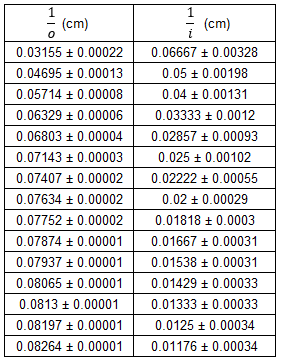
\includegraphics[width=0.8 \textwidth]{tablas/tabla espejo concavo.PNG}
    \captionof{table}{Distancias objeto e imagen obtenidos para el espejo cóncavo.}
    \label{fig}
\end{Figura}


\begin{Figura}
    \centering
    \includegraphics[width=1.15 \textwidth]{tablas/tabla tamaños espejo concavo.PNG}
    \captionof{table}{Distancias y tamaños objeto e imagen obtenidos para el espejo cóncavo y sus cocientes.}
    \label{fig}
\end{Figura}


\begin{Figura}
    \centering
    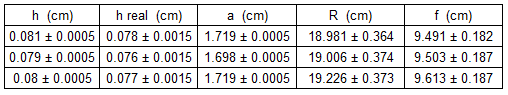
\includegraphics[width=1.1 \textwidth]{tablas/tabla esferometro.PNG}
    \captionof{table}{Distancias obtenidas con el esferómetro y radios y focos calculados.}
    \label{fig}
\end{Figura}




\end{multicols}
\end{document}
